\documentclass{article}
\setlength{\oddsidemargin}{0.25 in}
\setlength{\evensidemargin}{-0.25 in}
\setlength{\topmargin}{-0.6 in}
\setlength{\textwidth}{6.5 in}
\setlength{\textheight}{8.5 in}
\setlength{\headsep}{0.75 in}
\setlength{\parindent}{0 in}
\setlength{\parskip}{0.1 in}

% ===== PACKAGES =====
\usepackage{amsmath,amssymb}
\usepackage{color}
\usepackage{subfigure}
\usepackage{mdframed}
\usepackage{changepage}
\newmdenv[
  topline=false,
  bottomline=false,
  skipabove=\topsep,
  skipbelow=\topsep
]{siderules}
\renewcommand{\abstractname}{}

% ===== VARIABLES =====
\def \R{\mathbb{R}}
\def \Pr{\mathbb{P}}
\def \D{{\rm D}}
\def \N{{\rm N}}
\def \xx{{\boldsymbol{\rm x}}}
\def \y{{\rm y}}




% ===== HEADER BOX =====
\newcommand{\lecture}[2]{
\pagestyle{myheadings}
\thispagestyle{plain}
\newpage
\noindent
\begin{center}
\rule{\textwidth}{1.6pt}\vspace*{-\baselineskip}\vspace*{2pt} % Thick horizontal line
\rule{\textwidth}{0.4pt}\\[1\baselineskip] % Thin horizontal line
\vbox{\vspace{2mm}
\hbox to 6.28in { {\bf CS 760: Machine Learning} \hfill Spring 2024 }
\vspace{4mm}
\hbox to 6.28in { {\Large \hfill #1  \hfill} }
\vspace{4mm}
\hbox to 6.28in { {\scshape Authors:}  #2 \hfill }}
\vspace{-2mm}
\rule{\textwidth}{0.4pt}\vspace*{-\baselineskip}\vspace{3.2pt} % Thin horizontal line
\rule{\textwidth}{1.6pt}\\[\baselineskip] % Thick horizontal line
\end{center}
\vspace*{4mm}
}

% ===== Jed's Defined Stuff ======
\DeclareMathOperator*{\argmin}{arg\!\min}
\DeclareMathOperator*{\argmax}{arg\!\max}
\usepackage{siunitx}
\usepackage{enumitem} % used to make alphabetical lists instead of numbered ones
\usepackage{mathtools}
\usepackage{graphicx}
\usepackage{caption}
\usepackage{hyperref}


% =============== DOCUMENT ===============
\begin{document}
\lecture{Convolutional Neural Networks}{Jed Pulley \& Keshav Sharan Pachipala}

\begin{center}
{\Large {\sf \underline{\textbf{DO NOT POLLUTE!}} AVOID PRINTING, OR PRINT 2-SIDED MULTIPAGE.}}
\end{center}

% \begin{abstract}
% Write your abstract here
% \end{abstract}

\section{Introduction}
    In recent years, Convolutional Neural Networks (CNNs) have emerged as a cornerstone technology in the field of deep learning, particularly in the domain of computer vision. CNNs are adept at extracting intricate patterns and features from spatially structured data. Some fields that benefit from CNNs include:
        \begin{enumerate}
            \item Image Classification
            \item Object Detection
            \item Medical Image Analysis
        \end{enumerate}

\section{But What is a Convolution?}
    \subsection {The Discrete Case}
        Borrowing form the incredible 3Blue1Brown video example [1], let's say we want to roll a pair of dice and find the probability of seeing various different sums. You could visualize this as a grid where all six possibilities lie along the rows and columns, respectively: \\
        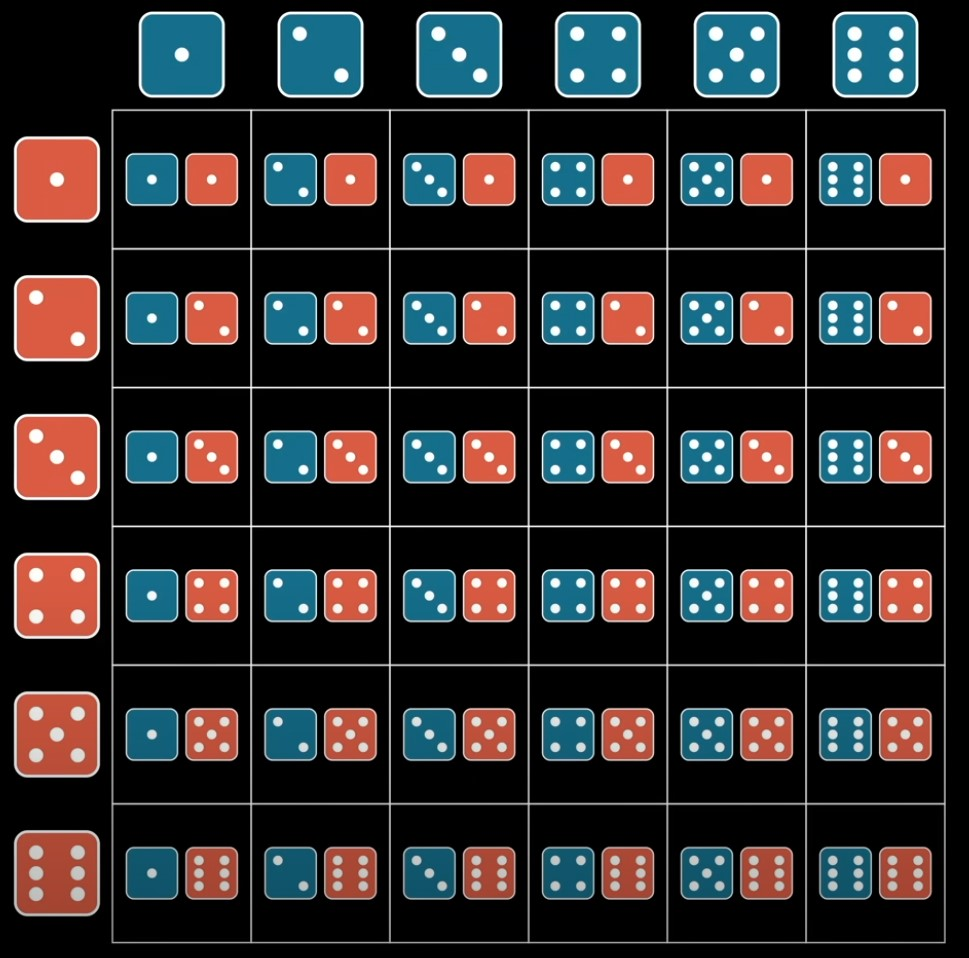
\includegraphics[scale=0.4]{images/dice-grid.jpg} \\
        To find this sum, we can just go along the diagonal and sum them up, giving us the total probability of finding that number. \\
        
        However, another way to illustrate this is by taking the six possibilities, listing them out, and flipping one set. This shows us all the possible combinations of the dice that sum to 7: \\
        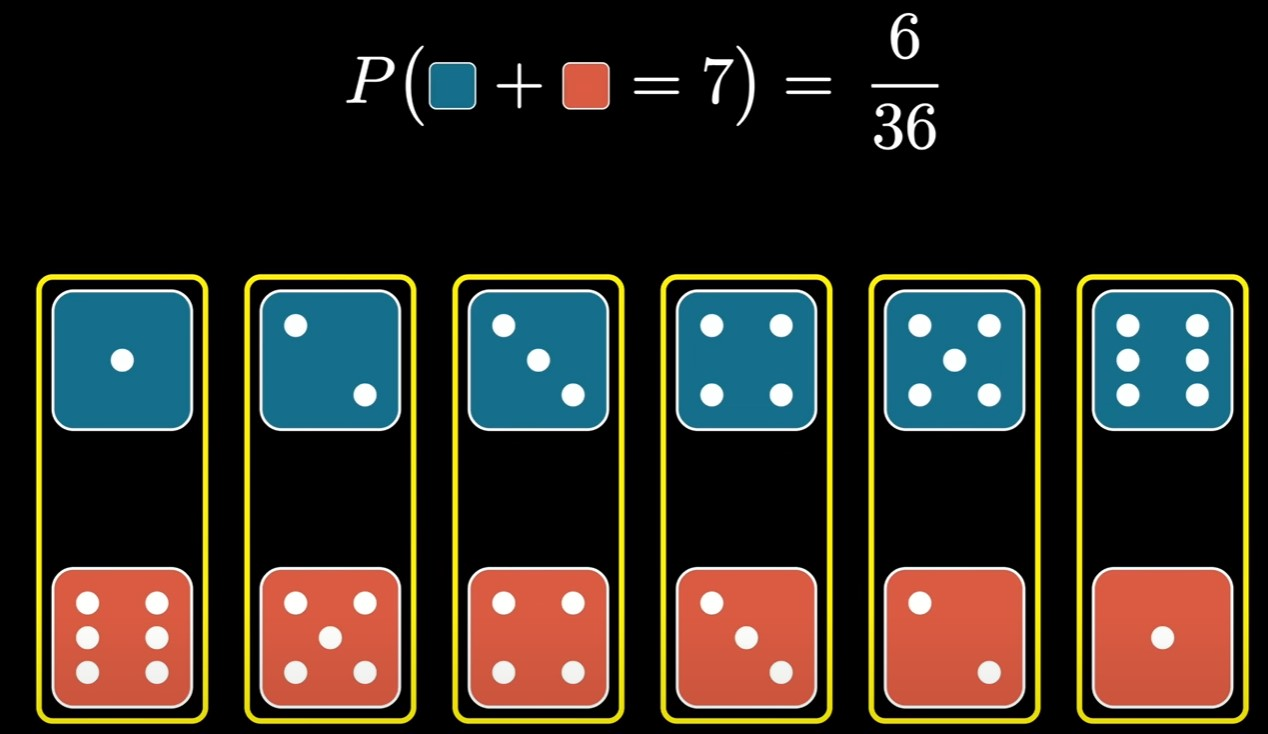
\includegraphics[scale=0.4]{images/flip.jpg} \\
        To find the rest of the sums, all we need to do is slide the bottom row of dice all the way to the left and then sum it up. We can slide the dice over each time to find the next sum: \\
        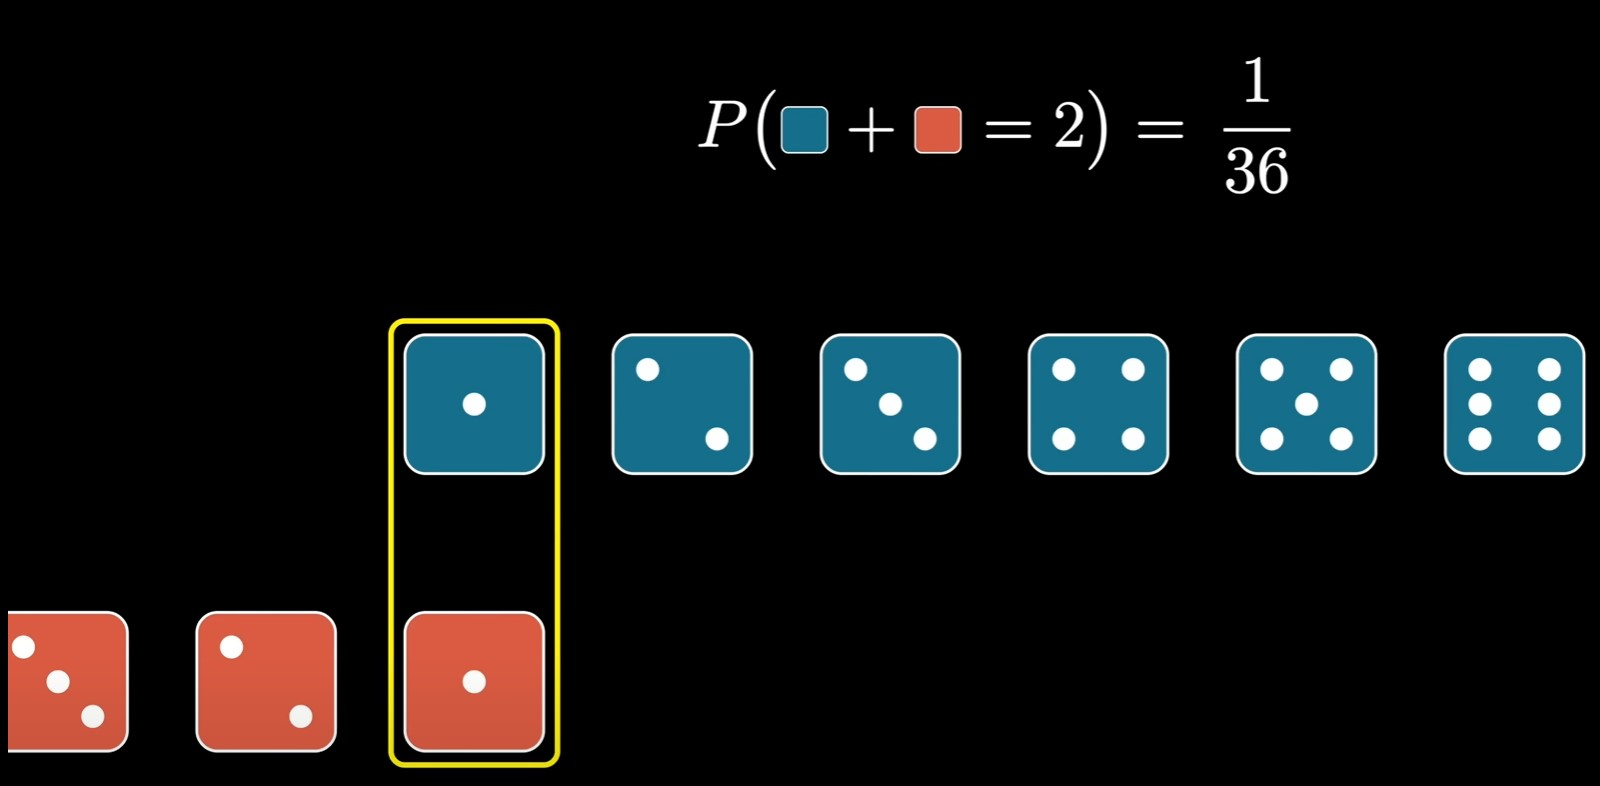
\includegraphics[scale=0.4]{images/slide.jpg} \\
        We can also change the weights of each dice to more align with the idea of finding the probability. But either way, this idea of taking two sequences, flipping one, and then adding them up to create a new sequence is called a \textbf{convolution}. In the 1D discrete case, we can write the formula for convolution as:
        \[(a * b)_n = \sum_{i,j} a_i \cdot b_i  \text{ such that } i + j = n\]
        
        Another good way to think of this is a moving average.

        \subsection {The Continuous Case}

\section{NNs vs CNNs}

\section{Understanding the Architecture}
    \subsection {Layers}
    \subsection {Feature Hierarchy}
    
\section{Advanced CNN Architectures}
    \begin{enumerate}[label=(\alph*)]
        \item VGGNet
        \item ResNet
        \item Inception Network
    \end{enumerate}
    
\section{Future Directions and Trends}
    \begin{enumerate}[label=(\alph*)]
        \item TO-DO
        \item TO-DO
        \item TO-DO
    \end{enumerate}

\section{Resources}
    \textbf{[1]} 3Blue1Brown - But What is a Convolution? \\
    \url{https://www.youtube.com/watch?v=KuXjwB4LzSA&t=1s}
    
    \textbf{[2]} 3Blue1Brown - Convolutions | Why X+Y in probability is a beautiful mess \\
    \url{https://www.youtube.com/watch?v=IaSGqQa5O-M}
    
    \textbf{[3]} far1din - Convolutional Neural Networks from Scratch | In Depth \\
    \url{https://www.youtube.com/watch?v=jDe5BAsT2-Y}
    
    \textbf{[4]} Younesi, A., Ansari, M., Fazli, M. A., Ejlali, A., Shafique, M., \& Henkel, J. (2024). A Comprehensive Survey of Convolutions in Deep Learning: Applications, Challenges, and Future Trends. arXiv preprint arXiv:2402.15490 \\
    \url{https://arxiv.org/abs/2402.15490}


\end{document} 